\documentclass[a4paper,10pt]{article}
%\documentclass[a4paper,10pt]{scrartcl}

\usepackage{xltxtra}

\setromanfont[Mapping=tex-text]{Droid Sans Fallback}
% \setsansfont[Mapping=tex-text]{DejaVu Sans}
% \setmonofont[Mapping=tex-text]{DejaVu Sans Mono}

\title{PosMeasure-WiFi无线测距(宿舍定位)}
\author{71112427 田宗耕}
\date{2015/6/28}

\begin{document}
\maketitle
  \section{PosMeasure项目介绍}
    \paragraph{} 本项目成品是一个安卓手机APP。它通过扫描多个wifi接入点的信号, 进行一定的处理,\\
    近似认为手机的位置就是信号最强AP的位置,从而绘制出自己在地图上的位置。
    \paragraph{} 本项目实现了我所在宿舍楼的5个宿舍房间的定位。
    \paragraph{} 地图如下:\\
    \begin{center} 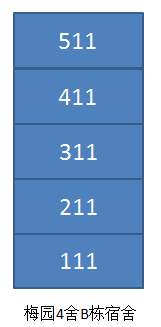
\includegraphics[width=1.60in,height=3.40in]{m4b.eps} \end{center}
  
  \section{实现思路}
    \subsection{接收WiFi无线信号}
    \paragraph{} 通过Andorid系统提供的API,可以得到当前手机连接到的WiFi接入点(AP)的MAC地址\\
    和信号强度等信息。由于宿舍区的无线信号种类很多,我进行了一次过滤,只收集名为\\
    “seu-wlan”的AP信息,存到一个数组中。然后找到信号强度最好的AP的MAC地址。
    \subsection{得到基本数据}
    \paragraph{} 我到地图中的5个宿舍房间门口进行测试,分别得到一个信号强度最好的AP的MAC地址。\\
    把地点和AP的MAC地址对应的信息存储到excel表中。
    \paragraph{} 因为宿舍区的WiFi信号特别不稳定,我特意选择了分别位于5个楼层走廊尽头的5个宿舍。
    \subsection{进行测试}
    \paragraph{} 实际使用时,APP会先得到信号最强的AP的MAC地址,然后和excel表中的数据进行比对,\\
    找出对应的地点信息。如果没有找到数据记录,则提示错误;如果找到了,则根据地点信息\\
    在地图上绘制出手机所在位置。
    
  \section{项目成品}
    \paragraph{}参见项目源码,以及附带的一个APK文件。
    
\end{document}
